% Options for packages loaded elsewhere
\PassOptionsToPackage{unicode}{hyperref}
\PassOptionsToPackage{hyphens}{url}
\PassOptionsToPackage{dvipsnames,svgnames,x11names}{xcolor}
%
\documentclass[
  11pt,
  ignorenonframetext,
]{beamer}
\usepackage{pgfpages}
\setbeamertemplate{caption}[numbered]
\setbeamertemplate{caption label separator}{: }
\setbeamercolor{caption name}{fg=normal text.fg}
\beamertemplatenavigationsymbolsempty
% Prevent slide breaks in the middle of a paragraph
\widowpenalties 1 10000
\raggedbottom
\setbeamertemplate{part page}{
  \centering
  \begin{beamercolorbox}[sep=16pt,center]{part title}
    \usebeamerfont{part title}\insertpart\par
  \end{beamercolorbox}
}
\setbeamertemplate{section page}{
  \centering
  \begin{beamercolorbox}[sep=12pt,center]{part title}
    \usebeamerfont{section title}\insertsection\par
  \end{beamercolorbox}
}
\setbeamertemplate{subsection page}{
  \centering
  \begin{beamercolorbox}[sep=8pt,center]{part title}
    \usebeamerfont{subsection title}\insertsubsection\par
  \end{beamercolorbox}
}
\AtBeginPart{
  \frame{\partpage}
}
\AtBeginSection{
  \ifbibliography
  \else
    \frame{\sectionpage}
  \fi
}
\AtBeginSubsection{
  \frame{\subsectionpage}
}
\usepackage{amsmath,amssymb}
\usepackage{lmodern}
\usepackage{setspace}
\usepackage{iftex}
\ifPDFTeX
  \usepackage[T1]{fontenc}
  \usepackage[utf8]{inputenc}
  \usepackage{textcomp} % provide euro and other symbols
\else % if luatex or xetex
  \usepackage{unicode-math}
  \defaultfontfeatures{Scale=MatchLowercase}
  \defaultfontfeatures[\rmfamily]{Ligatures=TeX,Scale=1}
\fi
% Use upquote if available, for straight quotes in verbatim environments
\IfFileExists{upquote.sty}{\usepackage{upquote}}{}
\IfFileExists{microtype.sty}{% use microtype if available
  \usepackage[]{microtype}
  \UseMicrotypeSet[protrusion]{basicmath} % disable protrusion for tt fonts
}{}
\makeatletter
\@ifundefined{KOMAClassName}{% if non-KOMA class
  \IfFileExists{parskip.sty}{%
    \usepackage{parskip}
  }{% else
    \setlength{\parindent}{0pt}
    \setlength{\parskip}{6pt plus 2pt minus 1pt}}
}{% if KOMA class
  \KOMAoptions{parskip=half}}
\makeatother
\usepackage{xcolor}
\geometry{left = 1cm, right = 0.5cm, top = 0.5cm, bottom = 0.5cm}
\newif\ifbibliography
\usepackage{color}
\usepackage{fancyvrb}
\newcommand{\VerbBar}{|}
\newcommand{\VERB}{\Verb[commandchars=\\\{\}]}
\DefineVerbatimEnvironment{Highlighting}{Verbatim}{commandchars=\\\{\}}
% Add ',fontsize=\small' for more characters per line
\usepackage{framed}
\definecolor{shadecolor}{RGB}{248,248,248}
\newenvironment{Shaded}{\begin{snugshade}}{\end{snugshade}}
\newcommand{\AlertTok}[1]{\textcolor[rgb]{0.94,0.16,0.16}{#1}}
\newcommand{\AnnotationTok}[1]{\textcolor[rgb]{0.56,0.35,0.01}{\textbf{\textit{#1}}}}
\newcommand{\AttributeTok}[1]{\textcolor[rgb]{0.77,0.63,0.00}{#1}}
\newcommand{\BaseNTok}[1]{\textcolor[rgb]{0.00,0.00,0.81}{#1}}
\newcommand{\BuiltInTok}[1]{#1}
\newcommand{\CharTok}[1]{\textcolor[rgb]{0.31,0.60,0.02}{#1}}
\newcommand{\CommentTok}[1]{\textcolor[rgb]{0.56,0.35,0.01}{\textit{#1}}}
\newcommand{\CommentVarTok}[1]{\textcolor[rgb]{0.56,0.35,0.01}{\textbf{\textit{#1}}}}
\newcommand{\ConstantTok}[1]{\textcolor[rgb]{0.00,0.00,0.00}{#1}}
\newcommand{\ControlFlowTok}[1]{\textcolor[rgb]{0.13,0.29,0.53}{\textbf{#1}}}
\newcommand{\DataTypeTok}[1]{\textcolor[rgb]{0.13,0.29,0.53}{#1}}
\newcommand{\DecValTok}[1]{\textcolor[rgb]{0.00,0.00,0.81}{#1}}
\newcommand{\DocumentationTok}[1]{\textcolor[rgb]{0.56,0.35,0.01}{\textbf{\textit{#1}}}}
\newcommand{\ErrorTok}[1]{\textcolor[rgb]{0.64,0.00,0.00}{\textbf{#1}}}
\newcommand{\ExtensionTok}[1]{#1}
\newcommand{\FloatTok}[1]{\textcolor[rgb]{0.00,0.00,0.81}{#1}}
\newcommand{\FunctionTok}[1]{\textcolor[rgb]{0.00,0.00,0.00}{#1}}
\newcommand{\ImportTok}[1]{#1}
\newcommand{\InformationTok}[1]{\textcolor[rgb]{0.56,0.35,0.01}{\textbf{\textit{#1}}}}
\newcommand{\KeywordTok}[1]{\textcolor[rgb]{0.13,0.29,0.53}{\textbf{#1}}}
\newcommand{\NormalTok}[1]{#1}
\newcommand{\OperatorTok}[1]{\textcolor[rgb]{0.81,0.36,0.00}{\textbf{#1}}}
\newcommand{\OtherTok}[1]{\textcolor[rgb]{0.56,0.35,0.01}{#1}}
\newcommand{\PreprocessorTok}[1]{\textcolor[rgb]{0.56,0.35,0.01}{\textit{#1}}}
\newcommand{\RegionMarkerTok}[1]{#1}
\newcommand{\SpecialCharTok}[1]{\textcolor[rgb]{0.00,0.00,0.00}{#1}}
\newcommand{\SpecialStringTok}[1]{\textcolor[rgb]{0.31,0.60,0.02}{#1}}
\newcommand{\StringTok}[1]{\textcolor[rgb]{0.31,0.60,0.02}{#1}}
\newcommand{\VariableTok}[1]{\textcolor[rgb]{0.00,0.00,0.00}{#1}}
\newcommand{\VerbatimStringTok}[1]{\textcolor[rgb]{0.31,0.60,0.02}{#1}}
\newcommand{\WarningTok}[1]{\textcolor[rgb]{0.56,0.35,0.01}{\textbf{\textit{#1}}}}
\setlength{\emergencystretch}{3em} % prevent overfull lines
\providecommand{\tightlist}{%
  \setlength{\itemsep}{0pt}\setlength{\parskip}{0pt}}
\setcounter{secnumdepth}{-\maxdimen} % remove section numbering
\titlegraphic{
\includegraphics[scale=0.05]{pictures/GlaLogo.pdf}}
\usepackage{float}
\usepackage{booktabs}
\usepackage{array}
\usepackage{longtable}
\setbeamertemplate{itemize item}{$\diamond$}
\setbeamertemplate{itemize subitem}{\scriptsize$\diamond$}
\setbeamertemplate{itemize subsubitem}{\scriptsize$\gg$}
\definecolor{blue}{RGB}{0,114,178}
\definecolor{red}{RGB}{213,94,0}
\definecolor{yellow}{RGB}{240,228,66}
\definecolor{green}{RGB}{0,158,115}
\ifLuaTeX
  \usepackage{selnolig}  % disable illegal ligatures
\fi
\IfFileExists{bookmark.sty}{\usepackage{bookmark}}{\usepackage{hyperref}}
\IfFileExists{xurl.sty}{\usepackage{xurl}}{} % add URL line breaks if available
\urlstyle{same} % disable monospaced font for URLs
\hypersetup{
  pdftitle={Introductory Statistics for Economics},
  pdfauthor={Duong Trinh},
  colorlinks=true,
  linkcolor={blue},
  filecolor={Maroon},
  citecolor={Blue},
  urlcolor={Blue},
  pdfcreator={LaTeX via pandoc}}

\title{Introductory Statistics for Economics}
\subtitle{ECON1013: TUTORIAL 3}
\author{Duong Trinh}
\date{Spring 2024}
\institute{University of Glasgow}

\begin{document}
\frame{\titlepage}

\setstretch{1.5}
\begin{frame}{Intro}
\protect\hypertarget{intro}{}
\begin{itemize}
\tightlist
\item
  Duong Trinh

  \begin{itemize}
  \tightlist
  \item
    PhD Student in Economics (Bayesian Microeconometrics)
  \item
    Email: \underline{Duong.Trinh@glasgow.ac.uk}
  \end{itemize}
\end{itemize}

\vspace{3mm}

\begin{itemize}
\tightlist
\item
  ECON1013-TU04

  \begin{itemize}
  \tightlist
  \item
    Monday 12-1 pm
  \item
    4 sessions (22-Jan, 5-Feb, 19-Feb, 4-March)
  \end{itemize}
\item
  ECON1013-TU05

  \begin{itemize}
  \tightlist
  \item
    Tuesday 12-1 pm
  \item
    4 sessions (23-Jan, 6-Feb, 20-Feb, 5-March)
  \end{itemize}
\item
  ECON1013-TU07

  \begin{itemize}
  \tightlist
  \item
    Tuesday 2-3 pm
  \item
    4 sessions (23-Jan, 6-Feb, 20-Feb, 5-March)
  \end{itemize}
\end{itemize}
\end{frame}

\begin{frame}{Record Attendance}
\protect\hypertarget{record-attendance}{}
\end{frame}

\hypertarget{brief-review}{%
\section{BRIEF REVIEW}\label{brief-review}}

\begin{frame}{BRIEF REVIEW}
\begin{center}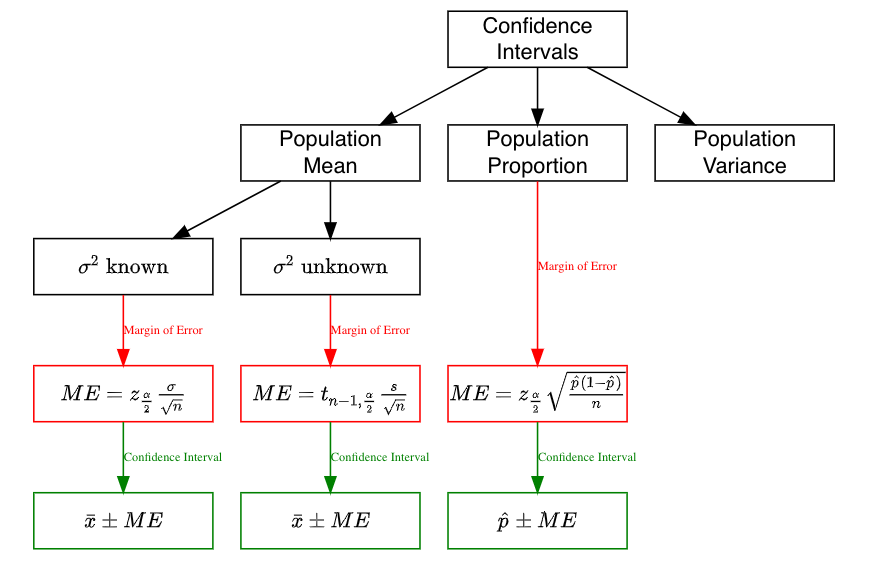
\includegraphics[width=0.9\linewidth]{pictures/CI_BriefReview} \end{center}
\end{frame}

\begin{frame}[fragile]{Exercise 1}
\protect\hypertarget{exercise-1}{}
\textbf{Redfield \& Wilton Strategies}

\begin{itemize}
\tightlist
\item
  Population Sampled: Eligible Voters in Scotland.
\item
  Sample Size: \(1,054\)
\item
  \(51\%\) of survey respondents now say they would vote
  ``\texttt{No}''.
\end{itemize}

\begin{enumerate}
[(a)]
\tightlist
\item
  Compute the margin of error (ME) of the proportion saying
  ``\texttt{No}'' at the \(95\%\) confidence level.
\item
  Compute the confidence interval at the \(95\%\) level.
\item
  Suppose I read from somewhere that the ME of that same survey is
  \(2.5\%\). Is this ME at a higher or at a lower confidence level?
\end{enumerate}
\end{frame}

\begin{frame}[fragile]{Exercise 1}
\protect\hypertarget{exercise-1-1}{}
\textbf{Ipsos}

\begin{itemize}
\tightlist
\item
  Population Sampled: Eligible Voters in Scotland.
\item
  Sample Size: \(1,004\)
\item
  54\% of voters back ``\texttt{Yes}'' \(\rightarrow\) The fraction for
  ``\texttt{No}'' in the Ipsos poll is \(0.46\).
\end{itemize}

\begin{enumerate}
[(a)]
\setcounter{enumi}{3}
\tightlist
\item
  Compute the margin of error (ME) of the proportion saying
  ``\texttt{No}'' at the \(95\%\) confidence level.
\item
  What is your view on the differences between the two polls?
\end{enumerate}
\end{frame}

\begin{frame}{Where are we in?}
\protect\hypertarget{where-are-we-in}{}
\begin{center}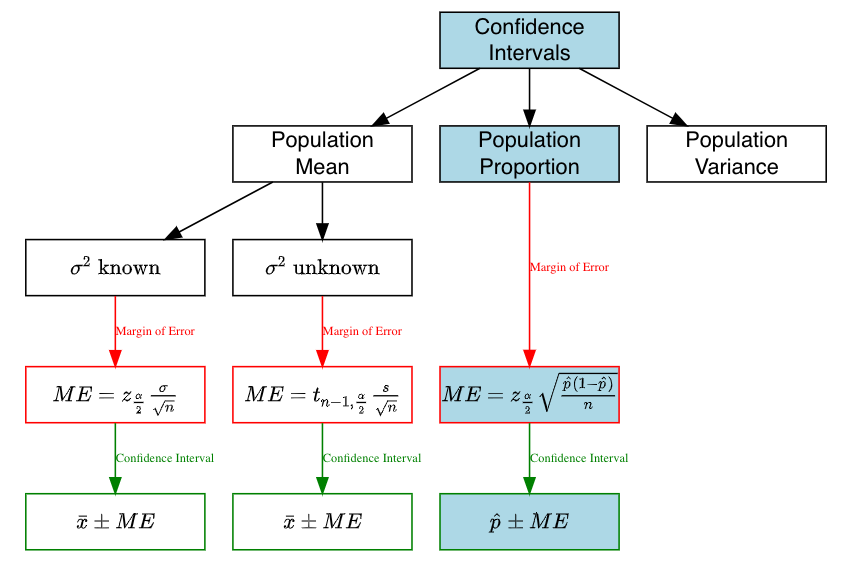
\includegraphics[width=0.9\linewidth]{pictures/CI_BriefReview-Ex1} \end{center}
\end{frame}

\begin{frame}[fragile]{(a) Compute the margin of error (ME) of the
proportion saying ``\texttt{No}'' at the \(95\%\) confidence level.}
\protect\hypertarget{a-compute-the-margin-of-error-me-of-the-proportion-saying-no-at-the-95-confidence-level.}{}
The formula for the margin of error for a population proportion
\(\hat{p}\) is given by

\[
\color{red}{ME = z_{\frac{\alpha}{2}} \sqrt{\frac{\hat{p}(1-\hat{p})}{n}}}
\]

\begin{itemize}
\tightlist
\item
  \(z_{\frac{\alpha}{2}}\): the value which cuts off
  \((\frac{\alpha}{2})\cdot 100\%\) of the probability mass in the right
  tail for a variable following a standard normal distribution.

  \begin{itemize}
  \tightlist
  \item
    Because the confidence level is \(1-\alpha=0.95\), we have that
    \(\alpha=0.05\) and \(\frac{\alpha}{2}=0.025\).
  \end{itemize}
\item
  Compute \(z_{0.025}\)

  \begin{itemize}
  \tightlist
  \item
    Looking at a statistical table: \(z_{0.025} = 1.96\), OR
  \item
    Using \texttt{Excel} function: \(=\text{NORM.INV}(0.975,0,1)\)
  \end{itemize}
\end{itemize}
\end{frame}

\begin{frame}{(a) Compute the margin of error (ME) of the proportion
saying ``\texttt{No}'' at the \(95\%\) confidence level.}
\protect\hypertarget{a-compute-the-margin-of-error-me-of-the-proportion-saying-no-at-the-95-confidence-level.-1}{}
Plugging in \(z_{0.025} = 1.96\), the sample size \(n = 1054\) and the
sample proportion \(\hat{p} = 0.51\), we find \[
ME = 1.96 \sqrt{\frac{0.51(1-0.51)}{1054}} = 1.96 \cdot{0.0153} \approx 0.03
\]

\(\Rightarrow\) The margin of error is approximately \(3\%\) at the
\(95\%\) confidence level.
\end{frame}

\begin{frame}{(b) Compute the confidence interval at the \(95\%\)
level.}
\protect\hypertarget{b-compute-the-confidence-interval-at-the-95-level.}{}
The confidence interval is given by \[
\hat{p} \pm ME
\]

\(0.51 \pm 0.03\) gives the interval \([0.48,0.54]\).
\end{frame}

\begin{frame}{(c) Suppose I read from somewhere that the ME of that same
survey is \(2.5\%\). Is this ME at a higher or at a lower confidence
level?}
\protect\hypertarget{c-suppose-i-read-from-somewhere-that-the-me-of-that-same-survey-is-2.5.-is-this-me-at-a-higher-or-at-a-lower-confidence-level}{}
\begin{itemize}
\tightlist
\item
  Confidence level = \(1-\alpha\)
\end{itemize}

\quad\quad\quad \(\alpha\) is smaller \(\Leftrightarrow\) Confidence
level is higher.

\begin{itemize}
\tightlist
\item
  \(ME = z_{\frac{\alpha}{2}} \sqrt{\frac{\hat{p}(1-\hat{p})}{n}}\)
\end{itemize}

\quad\quad\quad \(\alpha\) is smaller \(\Leftrightarrow\)
\(z_{\frac{\alpha}{2}}\) is \(\ldots\) \(\Leftrightarrow\) ME is
\(\ldots\).
\end{frame}

\begin{frame}{}
\protect\hypertarget{section}{}
If we compare \(z_{\frac{\alpha}{2}}\) for different values of
\(\alpha\), we see the following:

\(z_{\frac{0.10}{2}} = 1.64\),

\(z_{\frac{0.05}{2}} = 1.96\),

\(z_{\frac{0.01}{2}} = 2.58\),

We see that when \(\alpha\) is smaller, \(z_{\frac{\alpha}{2}}\) is
bigger.
\end{frame}

\begin{frame}{(c) Is this \(ME=2.5\%\) at a higher or at a lower
confidence level?}
\protect\hypertarget{c-is-this-me2.5-at-a-higher-or-at-a-lower-confidence-level}{}
\begin{itemize}
\tightlist
\item
  Confidence level = \(1-\alpha\)
\end{itemize}

\quad\quad\quad \(\alpha\) is smaller \(\Leftrightarrow\) Confidence
level is higher. \quad\quad  (1)

\begin{itemize}
\tightlist
\item
  \(ME = z_{\frac{\alpha}{2}} \sqrt{\frac{\hat{p}(1-\hat{p})}{n}}\)
\end{itemize}

\quad\quad\quad \(\alpha\) is smaller \(\Leftrightarrow\)
\(z_{\frac{\alpha}{2}}\) is bigger \(\Leftrightarrow\) ME is larger.
\quad  (2)

\pause

\begin{itemize}
\tightlist
\item
  From (1) and (2)
\end{itemize}

\quad\quad\quad \textcolor{red}{ME is larger}
\(\color{red}{\Leftrightarrow}\)
\textcolor{red}{Confidence level is higher.}

\pause

Since we found \(\text{ME} = 3\%\) at the \(95\%\) confidence level,
when ME is \(2.5\%\) (lower), the confidence level has to be
\textbf{lower}.
\end{frame}

\begin{frame}{(d) Compute the margin of error (ME) of the proportion
saying ``\texttt{No}'' at the \(95\%\) confidence level.}
\protect\hypertarget{d-compute-the-margin-of-error-me-of-the-proportion-saying-no-at-the-95-confidence-level.}{}
\pause

\begin{itemize}
\tightlist
\item
  The margin of error
\end{itemize}

\[
\color{red}{ME = z_{\frac{\alpha}{2}} \sqrt{\frac{\hat{p}(1-\hat{p})}{n}}}
\]

\[
\Rightarrow ME = 1.96 \sqrt{\frac{0.46(1-0.46)}{1004}} \approx 0.031
\]

\begin{itemize}
\tightlist
\item
  The \(95\%\) confidence level is approximately \([0.429,0.491]\).
\end{itemize}
\end{frame}

\begin{frame}{(e) What is your view on the differences between the two
polls?}
\protect\hypertarget{e-what-is-your-view-on-the-differences-between-the-two-polls}{}
\pause

\begin{itemize}
\item
  The confidence intervals are clearly different: \([0.429, 0.491]\) is
  different from \([0.48, 0.54]\), and in this sense, the estimates do
  differ.
\item
  However, at the same time, the intervals overlap (for example,
  \(49\%\) is contained in both), so they are not necessarily making
  different statements about the population parameter.
\item
  \textbf{Remark}: There exist statistical tests to determine whether
  \emph{two sample averages} are different from each other in a
  statistically significant way. We will learn about statistical testing
  procedures in Unit 5.
\end{itemize}
\end{frame}

\begin{frame}{Exercise 2}
\protect\hypertarget{exercise-2}{}
The government introduces a housing benefit of \(100\) pounds per month
for low-income households.

After the introduction of the policy, we collect a sample of rents paid
by \(31\) low-income households: \((r_1, r_2, \ldots , r_{31})\). In
this sample, the sample average rent is \(\bar{r} = 709\) pounds. In
this sample, the standard deviation is \(s_r = 34\).

\begin{enumerate}
[(a)]
\tightlist
\item
  Construct the margin of error for \(\bar{r}\).
\item
  Construct the \(95\%\) confidence interval for \(\bar{r}\).
\item
  We know that the average rent paid by low-income households, prior to
  the reform, was \(700\) pounds. Is this value, \(700\), still a likely
  population rent after the reform, based on the sample?
\end{enumerate}
\end{frame}

\begin{frame}{Where are we in?}
\protect\hypertarget{where-are-we-in-1}{}
\begin{center}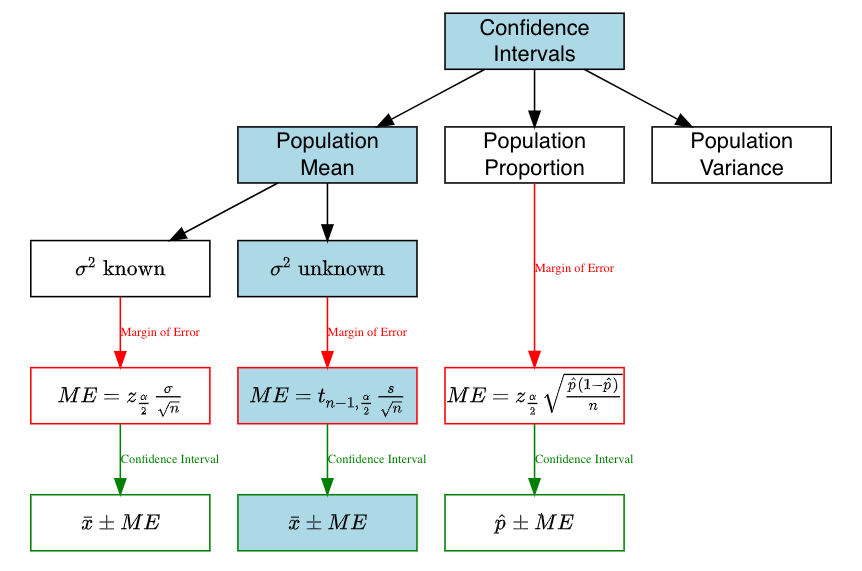
\includegraphics[width=0.9\linewidth]{pictures/CI_BriefReview-Ex2} \end{center}
\end{frame}

\begin{frame}[fragile]{(a) Construct the margin of error for
\(\bar{r}\).}
\protect\hypertarget{a-construct-the-margin-of-error-for-barr.}{}
The margin of error of the sample mean for a sample of size \(n\), when
the population standard deviation is not known, is given by

\[
\color{red}{ME = t_{n-1, \frac{\alpha}{2}} \frac{s}{\sqrt{n}}}
\]

\begin{itemize}
\tightlist
\item
  \(t_{n-1, \frac{\alpha}{2}}\): the value which cuts off
  \((\frac{\alpha}{2})\cdot 100\%\) of the probability mass in the right
  tail for a variable following a t-distribution with \(n-1\) degrees of
  freedom.

  \begin{itemize}
  \tightlist
  \item
    We use the Student's t distribution with \(n-1\) degrees of freedom.
  \item
    Because \(1-\alpha=0.95\), we have that \(\alpha=0.05\) and
    \(\frac{\alpha}{2}=0.025\).
  \end{itemize}
\item
  Calculate \(t_{30, 0.025}\):

  \begin{itemize}
  \tightlist
  \item
    Looking at a statistical table: \(t_{30, 0.025} = 2.042\), OR
  \item
    Using \texttt{Excel} function: \(=\text{T.INV}(0.975,30)\)
  \end{itemize}
\end{itemize}
\end{frame}

\begin{frame}{(a) Construct the margin of error for \(\bar{r}\).}
\protect\hypertarget{a-construct-the-margin-of-error-for-barr.-1}{}
Plugging in \(t_{30, 0.025} = 2.042\), the sample size \(n = 31\) and
the sample standard deviation \(s = 34\), we find

\[
ME = 2.042 \times \frac{34}{\sqrt{31}} \approx 12.47
\]
\end{frame}

\begin{frame}{(b) Construct the \(95\%\) confidence interval for
\(\bar{r}\).}
\protect\hypertarget{b-construct-the-95-confidence-interval-for-barr.}{}
\pause

\(\bar{r} =709\) \(\Rightarrow\) \(\bar{r} \pm 12.47\) give the
confidence interval \([696.5,721.5]\).
\end{frame}

\begin{frame}{(c) We know that the average rent paid by low-income
households, prior to the reform, was \(700\) pounds. Is this value,
\(700\), still a likely population rent after the reform, based on the
sample?}
\protect\hypertarget{c-we-know-that-the-average-rent-paid-by-low-income-households-prior-to-the-reform-was-700-pounds.-is-this-value-700-still-a-likely-population-rent-after-the-reform-based-on-the-sample}{}
\pause

\(700\) is contained in the \(95\%\) confidence interval. Therefore we
don't have very strong evidence suggesting that \(700\) is not a
possible value for the population mean after the reform, at the \(95\%\)
confidence level.
\end{frame}

\hypertarget{excel-note}{%
\section{EXCEL NOTE}\label{excel-note}}

\begin{frame}[fragile]{Relevant functions (I)}
\protect\hypertarget{relevant-functions-i}{}
\normalsize

Launch the \textbf{Excel} online

\footnotesize

\textcolor{blue}{https://www.office.com/launch/excel?auth=2}

\vspace{3mm}

\normalsize

\textcolor{red}{NORM.INV()} \footnotesize To return the inverse of the
normal cumulative distribution for the specified mean and standard
deviation (\emph{real number}).

\begin{Shaded}
\begin{Highlighting}[]
\NormalTok{= NORM.INV(probability,mean,standard\_dev)}
\end{Highlighting}
\end{Shaded}

\normalsize

\textcolor{red}{T.INV()} \footnotesize To return the t-value of the
Student's t-distribution as a function of the probability and the
degrees of freedom (\emph{real number}).

\begin{Shaded}
\begin{Highlighting}[]
\NormalTok{= T.INV(probability,degrees\_freedom)}
\end{Highlighting}
\end{Shaded}
\end{frame}

\begin{frame}[fragile]{Relevant functions (II)}
\protect\hypertarget{relevant-functions-ii}{}
\normalsize

Launch the \textbf{Excel} online

\footnotesize

\textcolor{blue}{https://www.office.com/launch/excel?auth=2}

\vspace{3mm}

\normalsize

\textcolor{red}{NORMSDIST()} \footnotesize To return the standard normal
cumulative distribution (\emph{probability}).

\begin{Shaded}
\begin{Highlighting}[]
\NormalTok{= NORMSDIST(z)}
\end{Highlighting}
\end{Shaded}
\end{frame}

\end{document}
